% ---------------------------------------------------------------------------
\section{Exploratory Data Analysis}
\label{sec:eda}
% ---------------------------------------------------------------------------

\subsection{The distribution of sale price}

Figure~\ref{fig:price-dist} shows the target before and after transformation. The
raw distribution is unimodal and strongly right-skewed, with a long tail above
400,000 \USD{} and a skewness of 1.881. The mean (180,933 \USD) sits 17,933 \USD{}
above the median (163,000 \USD), visible in the figure as the separation between the
reference lines. The natural logarithm reduces skewness to 0.122 and kurtosis from
6.52 to 0.80, compressing the influence of extreme observations without discarding
them. The transformation is not a complete cure: a Shapiro--Wilk test on the logged
target rejects normality ($p = 1.2\times10^{-7}$), which matters because a model
assuming Gaussian errors in log space would produce intervals that are too narrow in
the tails. This is one reason the project adopts conformal rather than analytical
intervals.

\begin{figure}[htbp]
\centering
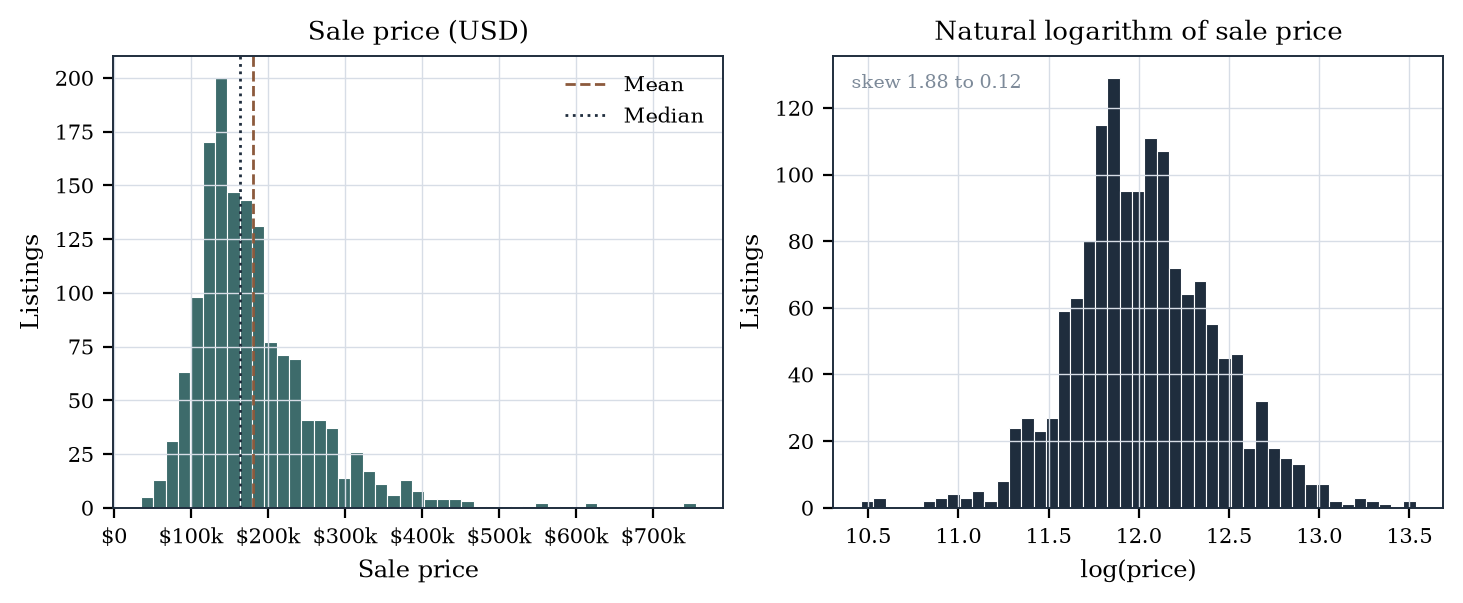
\includegraphics[width=0.90\linewidth]{fig01_price_distribution.png}
\caption{Sale price in \USD{} (left) and its natural logarithm (right). The dashed
and dotted rules mark the mean and median. Logarithmic scaling reduces skewness from
1.881 to 0.122.}
\label{fig:price-dist}
\end{figure}

\subsection{Location and sub-market segmentation}

Location is the strongest organising structure in the data.
Figure~\ref{fig:neigh} orders the 25 neighbourhoods by median price and shows
substantial separation. The median ranges from 88,000 \USD{} in MeadowV and 103,000
\USD{} in IDOTRR to 301,500 \USD{} in NoRidge and 315,000 \USD{} in NridgHt, a ratio
of more than three to one within one small city. The ordering matches local
knowledge: newer northern and western neighbourhoods with larger lots sit at the top,
older eastern and southern neighbourhoods at the bottom.

\begin{figure}[htbp]
\centering
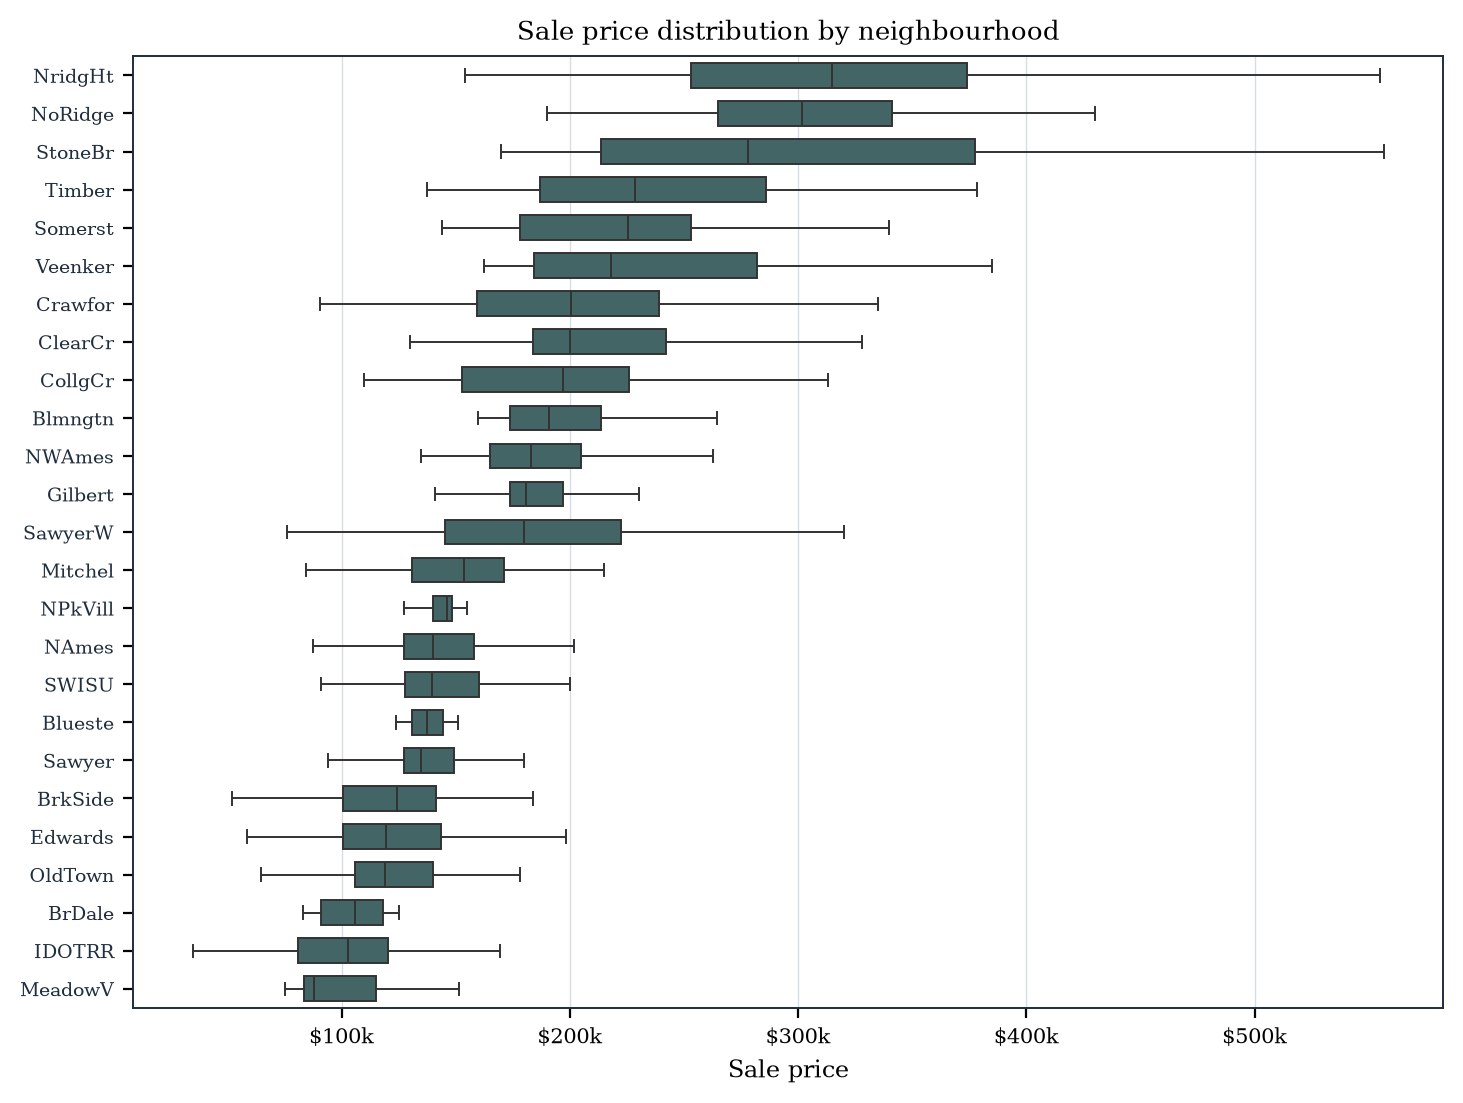
\includegraphics[width=0.60\linewidth]{fig02_price_by_neighbourhood.png}
\caption{Distribution of sale price by neighbourhood, ordered by median. Boxes span
the interquartile range, the central rule marks the median, and whiskers extend to
1.5 times the interquartile range.}
\label{fig:neigh}
\end{figure}

Aggregating the neighbourhoods into five tiers, the prior used by the synthetic
generator, produces a monotone gradient in median price: 109,000 \USD{} for tier 1,
125,500 for tier 2, 148,000 for tier 3, 196,750 for tier 4 and 306,000 for tier 5.
The gradient is not an artefact of the tier construction, because the tier never
enters the model; it is a compact description of how much price variation in this
market is locational. It also implies that a single global error metric will hide
large differences in dollar error across sub-markets, a point developed in
Section~\ref{sec:models}.

\subsection{Property type, architectural style and age}

Property type adds a dimension that location alone does not capture.
Single-family detached homes dominate with 1,218 of 1,458 transactions and a median
of 167,900 \USD. Attached end units (TwnhsE, 114 listings) have a near-identical
median of 172,200 \USD, whereas interior townhouses (43 listings, median 137,500
\USD), duplexes (52 listings, 135,980 \USD) and conversions (2fmCon, 31 listings,
127,500 \USD) trade at a discount of roughly 18 to 24 per cent to detached stock
(Figure~\ref{fig:ptype}). Two-storey homes (443 listings, median 190,000 \USD) and
split levels (65 listings, 164,500 \USD) sit above single-storey homes (726 listings,
154,750 \USD). Style is partly a proxy for size and vintage, so its marginal effect
should not be read as a causal premium for height; the practical consequence is that
the listing profile must include building type and style, because pricing a duplex
with a detached-home template would systematically over-value it.

\begin{figure}[htbp]
\centering
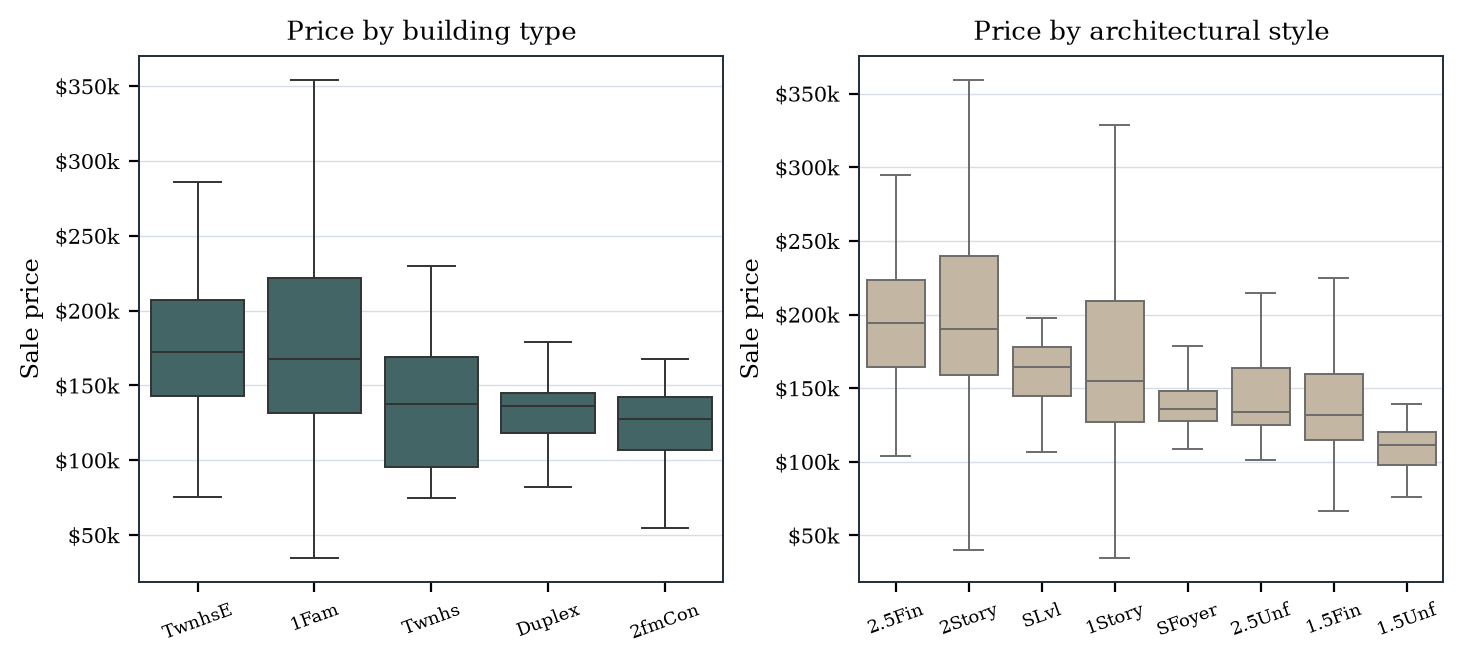
\includegraphics[width=0.88\linewidth]{fig25_price_by_property_type.png}
\caption{Sale price by building type (left) and architectural style (right). Detached
single-family homes and two-storey styles occupy the upper part of the distribution;
interior townhouses, duplexes and conversions occupy the lower part.}
\label{fig:ptype}
\end{figure}

Age is negatively associated with price at the margin: age at sale correlates at
$-0.524$ and years since remodelling at $-0.510$. The relationship is not monotone
across construction cohorts (Table~\ref{tab:decade}). Median prices rise from 108,000
\USD{} for the 1870s cohort to 224,000 \USD{} for the 2000s cohort, but the 1920s
cohort (115,000 \USD) is cheaper than the 1910s cohort (128,750 \USD), and median
floor area rises from around 1,200--1,300 square feet in the mid-twentieth century to
1,636 square feet in the 2000s. Part of the apparent age premium is therefore a size
premium, and the multivariate model is needed to separate the two. Renovation is a
separate signal: the scope indicator correlates negatively with price ($-0.199$)
because deep renovations concentrate in the oldest stock, where a major renovation is
evidence that a house needed one.

\begin{table}[htbp]
\centering
\caption{Sale price and floor area by construction decade, selected cohorts. The 2010
cohort contains a single transaction and is reported for completeness only.}
\label{tab:decade}
\small
\begin{tabular}{@{}lrrr@{}}
\toprule
\textbf{Construction decade} & \textbf{Listings} & \textbf{Median price (\USD)} & \textbf{Median area (sqft)} \\
\midrule
1870s & 2 & 108,000 & 1,689 \\
1910s & 58 & 128,750 & 1,566 \\
1920s & 97 & 115,000 & 1,208 \\
1950s & 167 & 136,000 & 1,196 \\
1970s & 188 & 147,500 & 1,273 \\
1990s & 163 & 204,000 & 1,716 \\
2000s & 385 & 224,000 & 1,636 \\
2010 & 1 & 394,432 & 1,856 \\
\bottomrule
\end{tabular}
\end{table}

\subsection{Price drivers, amenity access and collinearity}

Figure~\ref{fig:corr} ranks the marginal correlations with price. Size and quality
dominate: total floor area (0.833), overall quality (0.796), above-grade living area
(0.735), basement area (0.651) and garage capacity (0.641) are the strongest positive
associates, while the crime index ($-0.551$), age at sale ($-0.524$) and distance to
transit ($-0.365$) are the strongest negative ones. The pattern is economically
sensible: buyers pay for space, condition and access, and discount distance and
disamenity.

\begin{figure}[htbp]
\centering
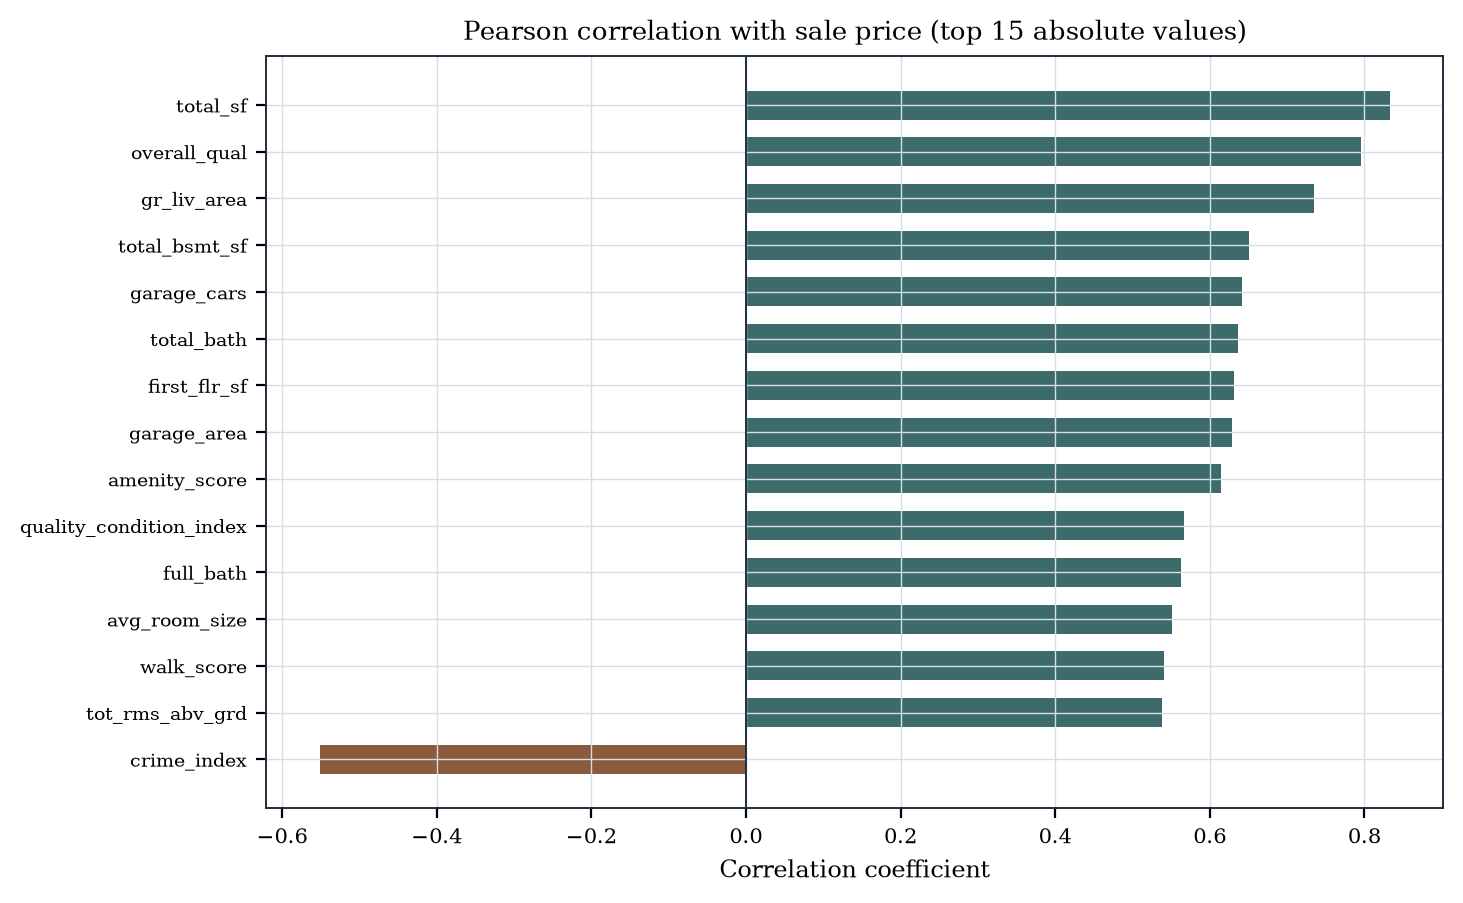
\includegraphics[width=0.88\linewidth]{fig03_price_drivers_correlation.png}
\caption{Pearson correlation of the fifteen attributes most strongly associated with
sale price. Positive associations are dark green, negative associations brown. The
ranking is descriptive and ignores confounding between attributes.}
\label{fig:corr}
\end{figure}

Figure~\ref{fig:amenity} makes the location gradient explicit. Premium neighbourhoods
cluster at high amenity scores and high prices, value neighbourhoods at low scores and
low prices, and the overlap region is where the model earns its keep: properties with
similar amenity access but different structural quality must be separated by the
structural attributes. The figure also exposes heteroscedasticity: the vertical spread
of price at a given amenity score rises from roughly 50,000 \USD{} in the value
segment to more than 300,000 \USD{} in the premium segment. Absolute errors will
therefore be larger for expensive homes even when relative errors are comparable,
which is why the evaluation reports both dollar and percentage errors and why
interval width is expressed as a percentage of the estimate.

\begin{figure}[htbp]
\centering
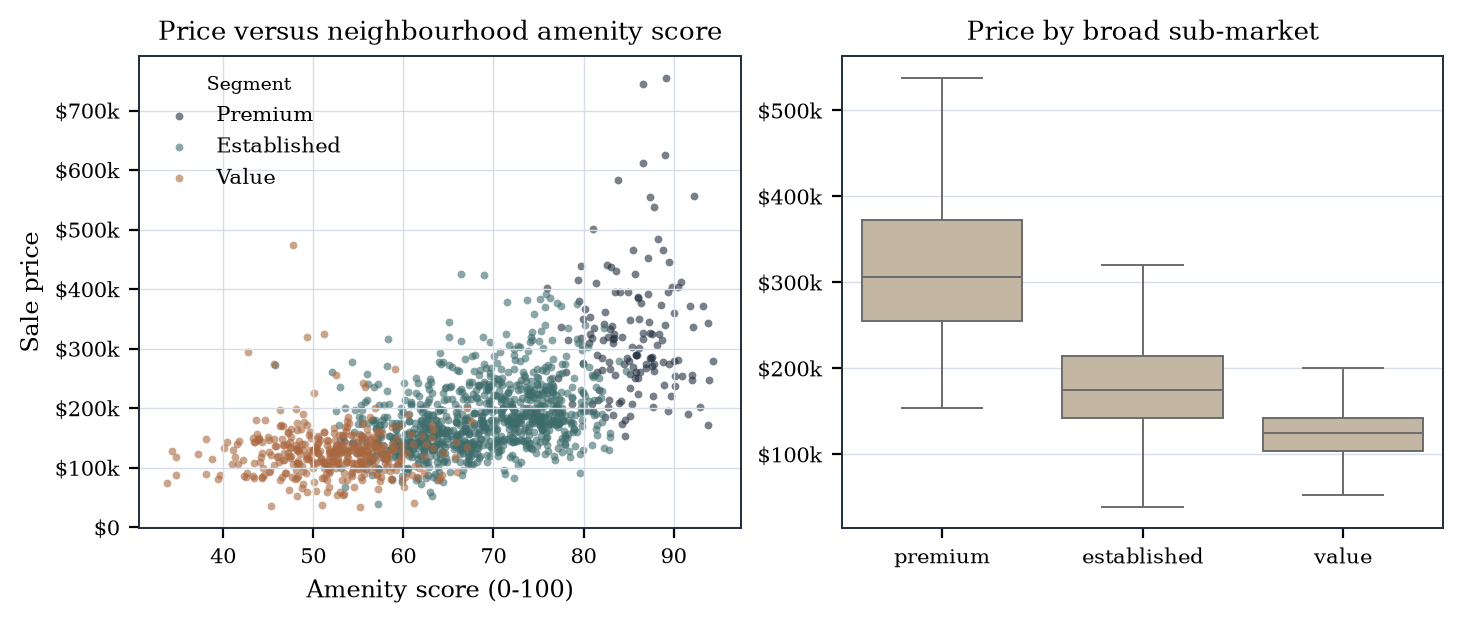
\includegraphics[width=0.88\linewidth]{fig05_amenity_price.png}
\caption{Price against neighbourhood amenity score by sub-market segment (left) and
price within the three segments (right). The association is positive and
heteroscedastic.}
\label{fig:amenity}
\end{figure}

Marginal correlations are a screening device, not a model. Total floor area is a
composite of basement, first-floor and second-floor areas and correlates with
above-grade living area at 0.866; garage area and capacity correlate at 0.887;
construction year and age at sale correlate at $-0.999$ by construction. These
redundancies inflate variance inflation factors and destabilise linear coefficients,
which motivates the pruning described in Section~\ref{sec:features}.
